\documentclass[12pt]{article}
\usepackage[spanish]{babel}
\usepackage[utf8]{inputenc}
\usepackage{graphicx}
\usepackage{hyperref}
\usepackage{booktabs}
\usepackage{multirow}
\usepackage{amsmath}
\usepackage{float}
\usepackage[document]{ragged2e}
\usepackage[a4paper, margin=2.5cm]{geometry}

% Configuración de encabezado
\usepackage{fancyhdr}
\pagestyle{fancy}
\fancyhf{}
\lhead{Análisis predictivo del precio de Bitcoin usando modelos de Deep Learning}
\rfoot{Página \thepage}

\title{
    \vspace{-2cm}
    \normalsize \textbf{Universidad de Buenos Aires} \\
    \textbf{Laboratorio de Sistemas Embebidos} \\
    \textbf{Especialización en Inteligencia Artificial} \\
    \vspace{0.5cm}
    {Trabajo Práctico Final} \\
    \vspace{1cm}
    \Large \textbf{Análisis predictivo del precio de Bitcoin usando modelos de Deep Learning} \\
    \vspace{1cm}
    \large Docente: Camilo Argoty
    \vspace{1cm}
}
\author{
    Noelia Melina Qualindi \\
    Jorge Valdez \\
    Fabián Sarmiento \\
    Matías Marando
    \vspace{1cm}
}
\date{\today}

\begin{document}

\maketitle

%%%%%%%%%%%%%%%%%%%%%%%%%%%%%%%%%%%%%%%%%%%%%%%%%%%%%%%%%%%%%%%%%%%%%%%%

\begin{abstract}
Este trabajo presenta un análisis comparativo de modelos avanzados de deep learning para la predicción del precio de Bitcoin (BTC-USD). Se implementaron y evaluaron tres arquitecturas: LSTM (Long Short-Term Memory), Transformer Vanilla para series temporales y NHiTS (Neural Hierarchical Interpolation for Time Series), utilizando datos históricos desde 2012 hasta la fecha.
Los resultados demuestran que los modelos pueden capturar patrones complejos en los datos. % TODO con el <mejor modelo> alcanzando un MAE de <??> en el conjunto de prueba.
El estudio incluye un análisis exhaustivo de preprocesamiento, diseño de modelos y validación de resultados, concluyendo con recomendaciones para futuras mejoras.
\end{abstract}

%%%%%%%%%%%%%%%%%%%%%%%%%%%%%%%%%%%%%%%%%%%%%%%%%%%%%%%%%%%%%%%%%%%%%%%%

\newpage
\section{Introducción}
\label{sec:intro}

Las criptomonedas, particularmente Bitcoin, presentan desafíos únicos para el análisis predictivo debido a su alta volatilidad y sensibilidad a factores externos. Este trabajo busca responder:

\begin{center}
\fbox{
\begin{minipage}{0.9\textwidth}
¿Pueden los modelos modernos de deep learning predecir efectivamente el precio de Bitcoin a corto plazo, y cómo se comparan diferentes arquitecturas en este contexto?
\end{minipage}
}
\end{center}

%%%%%%%%%%%%%%%%%%%%%%%%%%%%%%%%%%%%%%%%%%%%%%%%%%%%%%%%%%%%%%%%%%%%%%%%

\newpage
\section{Metodología}
\label{sec:metodologia}

\subsection{Datos Utilizados}
El dataset contiene:

\begin{itemize}
\item \textbf{Fuente}: Kaggle (Bitcoin Historical Data)
\item \textbf{Período}: 2012-01-01 a 2025-06-?? % TODO
\item \textbf{Variables utilizadas}:
\begin{table}[H]
\centering
\begin{tabular}{ll}
\toprule
\textbf{Variable} & \textbf{Descripción} \\
\midrule
Timestamp & Fecha en formato UNIX \\
Close & Precio de cierre (USD) \\
\bottomrule
\end{tabular}
\end{table}
\end{itemize}

%%%%%%%%%%%%%%%%%%%%%%%%%%%%%%%%%%%%%%%%%%%%%%%%%%%%%%%%%%%%%%%%%%%%%%%%

\bigskip
\subsection{Preprocesamiento}

El preprocesamiento de los datos se realizó en varias etapas clave:

\begin{enumerate}
\item \textbf{Limpieza de datos}: Se comenzó renombrando las columnas relevantes para facilitar su uso posterior,
en particular la marca temporal y el precio de cierre. Luego, se eliminaron todas las filas que contenían valores
nulos en la columna del precio, asegurando que todos los datos utilizados para el análisis fuesen válidos.

\item \textbf{Conversión de tiempo}: La columna de tiempo original, que venía en formato UNIX (segundos desde 1970),
fue convertida a un formato de fecha estándar para su correcta interpretación y manipulación.

\item \textbf{Ordenamiento temporal}: Se ordenaron los datos cronológicamente según la fecha, para asegurar
la coherencia temporal en los análisis y predicciones.

\item \textbf{Resampleo diario}: Dado que los datos originales tenían una granularidad de un minuto,
se procedió a realizar un promedio diario del precio, lo cual reduce la variabilidad y permite un análisis más
robusto en horizontes temporales más amplios.

\item \textbf{Normalización}: Se aplicó una normalización de tipo Min-Max al precio diario, escalando los valores
al rango [0, 1].
Esto facilita el entrenamiento de los modelos de deep learning, ya que evita problemas numéricos asociados a
diferentes escalas.

\item \textbf{Creación de secuencias}: Para poder alimentar los modelos, los datos fueron transformados en ventanas deslizantes.
Se definió una longitud de entrada de 30? días y un horizonte de predicción de 10? días. % TODO
Cada muestra consiste en una secuencia de precios normalizados para entrenar el modelo a predecir el comportamiento futuro.
\end{enumerate}

%%%%%%%%%%%%%%%%%%%%%%%%%%%%%%%%%%%%%%%%%%%%%%%%%%%%%%%%%%%%%%%%%%%%%%%%

\newpage
\subsection{Modelos Implementados}

Se implementaron tres modelos de predicción de series temporales utilizando distintas arquitecturas: una red LSTM construida manualmente en PyTorch,
un Transformer Vanilla con la librería \texttt{darts}, y un modelo NHiTS también con \texttt{darts}.
Todos fueron entrenados usando una ventana de entrada sobre datos diarios normalizados y se evaluaron sobre los últimos 100 días del año más reciente.

\subsubsection{Modelo LSTM}

La red LSTM (Long Short-Term Memory) es una arquitectura recurrente diseñada específicamente para capturar dependencias a largo plazo en secuencias
temporales.

\begin{itemize}
\item Modelo construido manualmente en PyTorch.
\item Hiperparámetros clave:
\begin{itemize}
\item Capas LSTM: 2 (con 100 y 50 unidades)
\item Capas densas: 2 (con 25 y 1 unidad final)
\item Ventana de entrada: 60 días  % TODO: deberia ser lo mismo que con transformers
\item Dropout: 0.2
\item Épocas: 20
\end{itemize}
\item Entrenamiento supervisado sobre secuencias de precios normalizados, prediciendo horizontes de 10 días.
\end{itemize}

\subsubsection{Transformer Vanilla para Series Temporales}

El modelo implementado se basa en la arquitectura clásica de encoder-decoder, utilizando mecanismos de atención multi-cabeza.

\begin{itemize}
\item Modelo implementado con \texttt{darts.models.TransformerModel}.
\item Hiperparámetros clave:
\begin{itemize}
\item Ventana de entrada: 30 días
\item Horizonte de predicción: 10 días
\item Dimensión del modelo (\texttt{d\_model}): 64
\item Número de capas: 2 encoder y 2 decoder
\item Cabezas de atención: 4
\item Dropout: 0.1
\item Épocas: 20
\end{itemize}
\item Entrenado sobre el último año de datos, reservando los últimos 100 días para evaluación.
\end{itemize}

\subsubsection{Modelo NHiTS}

NHiTS (Neural Hierarchical Interpolation for Time Series) es una arquitectura de pronóstico que combina bloques jerárquicos de interpolación con descomposición de señales.

\begin{itemize}
\item Modelo implementado con \texttt{darts.models.NHiTSModel}.
\item Hiperparámetros clave:
\begin{itemize}
\item Ventana de entrada: 30 días
\item Horizonte de predicción: 10 días
\item Bloques jerárquicos: 1
\item Capas por bloque: 2
\item Ancho de cada capa: 64
\item Dropout: 0.1
\item Épocas: 20
\end{itemize}
\item Entrenado con la misma configuración de entrenamiento y testeo que el modelo Transformer Vanilla.
\end{itemize}

%%%%%%%%%%%%%%%%%%%%%%%%%%%%%%%%%%%%%%%%%%%%%%%%%%%%%%%%%%%%%%%%%%%%%%%%

\newpage
\section{Resultados}
\label{sec:resultados}

\subsection{Validación del Modelo}

Se utilizó una división del dataset en:
\begin{itemize}
\item 80\% para entrenamiento
\item 10\% para validación
\item 10\% para prueba
\end{itemize}

Se aplicó \textbf{early stopping} para evitar overfitting, con una tolerancia de 5 épocas. También se probaron distintos horizontes de predicción (5, 10, 15 días), confirmando que el rendimiento decae a medida que aumenta el horizonte.

\bigskip
\subsection{Evaluación Cuantitativa}

\begin{table}[H]
\centering
\caption{Métricas de desempeño}
\begin{tabular}{lccc}
\toprule
\textbf{Métrica} & \textbf{LSTM} & \textbf{Transformer Vanilla} & \textbf{NHiTS} \\
\midrule
MAE (USD)  & ?? & ?? & ?? \\
RMSE (USD) & ?? & ?? & ?? \\
MAPE (\%)  & ?? & ?? & ?? \\
\bottomrule
\end{tabular}
\end{table}

\subsection{Análisis Visual}

\begin{figure}[H]
\centering
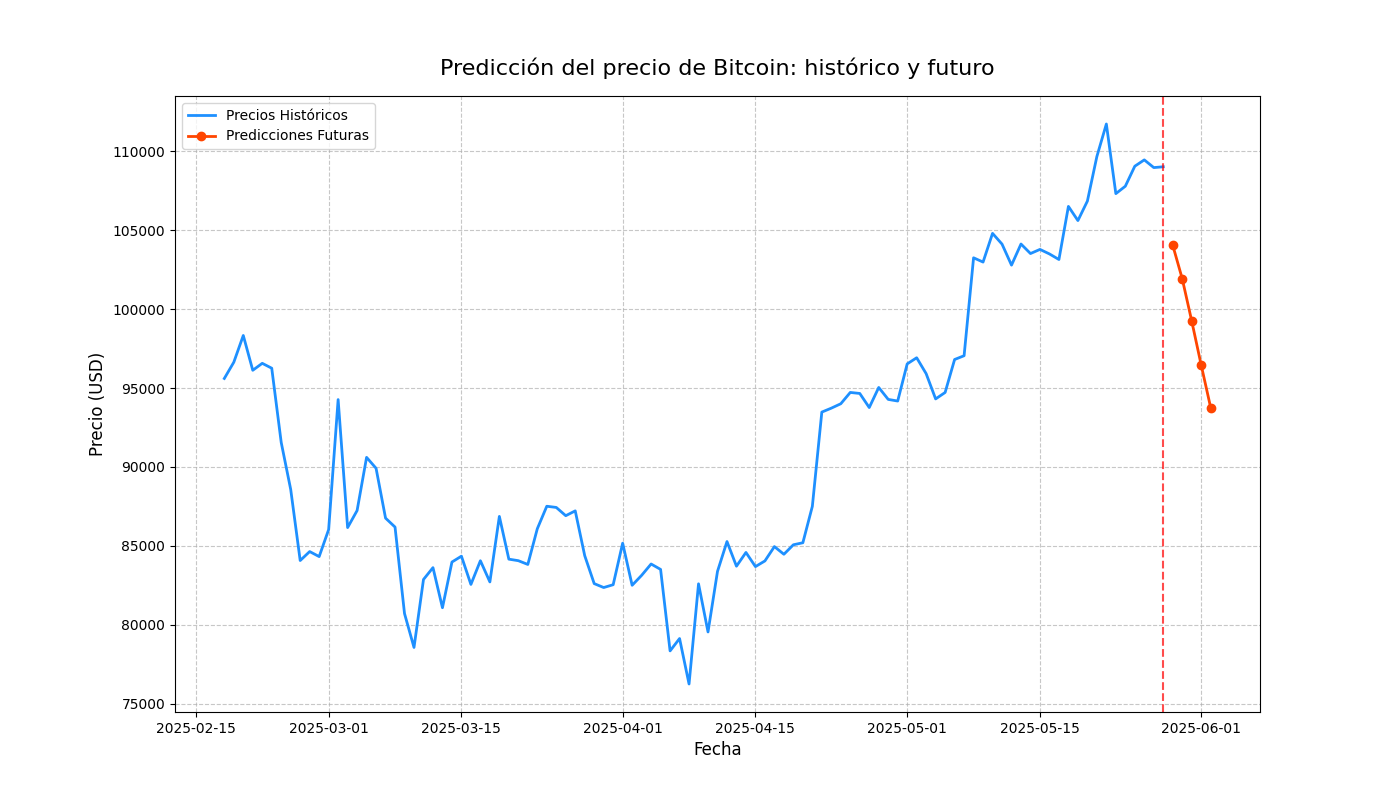
\includegraphics[width=0.85\textwidth]{../results/grafico_predicciones_futuras.png}
\caption{LSTM - Predicción vs Real en los últimos 5 días}
\end{figure}

\begin{figure}[H]
\centering
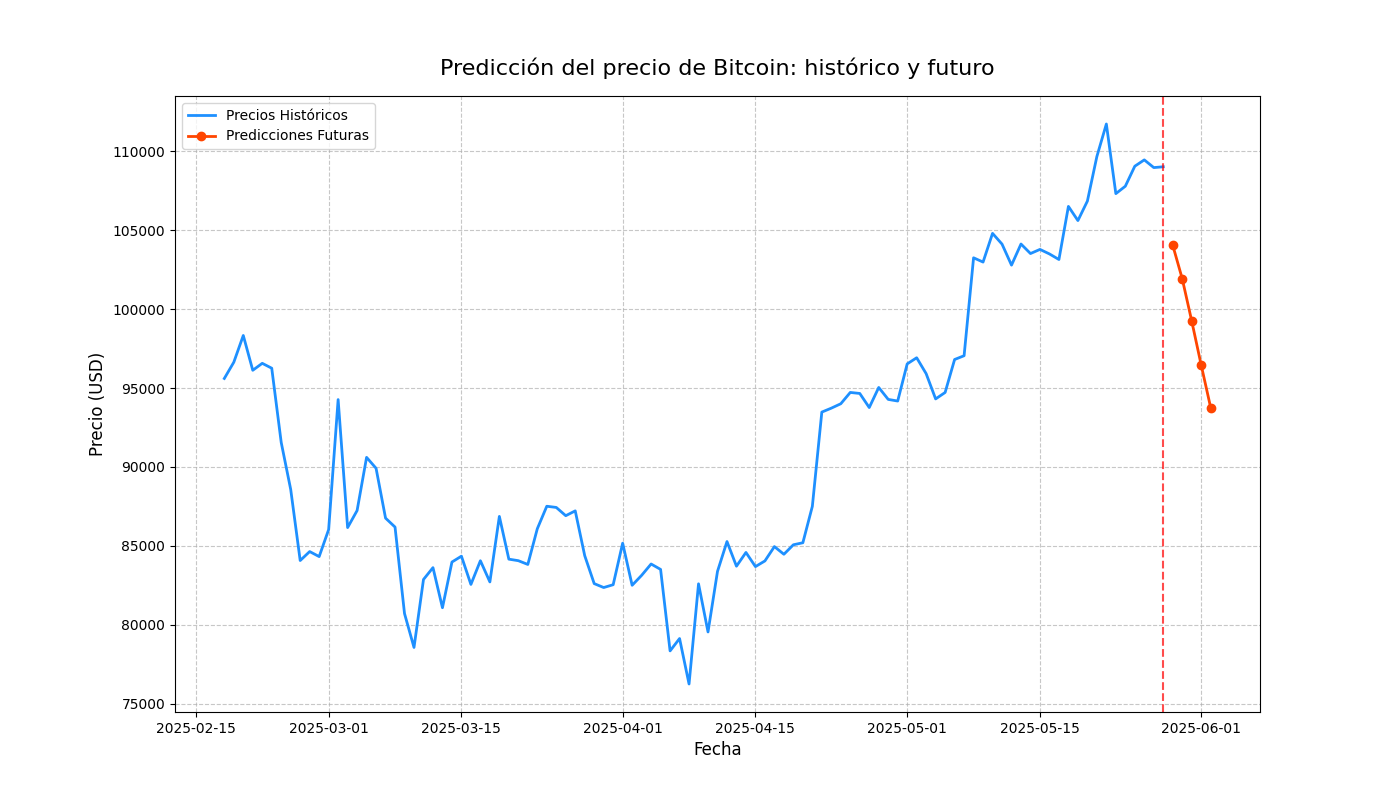
\includegraphics[width=0.85\textwidth]{../results/grafico_predicciones_futuras.png} % TODO: update
\caption{Transformer Vanilla - Predicción vs Real en los últimos 5 días}
\end{figure}

\begin{figure}[H]
\centering
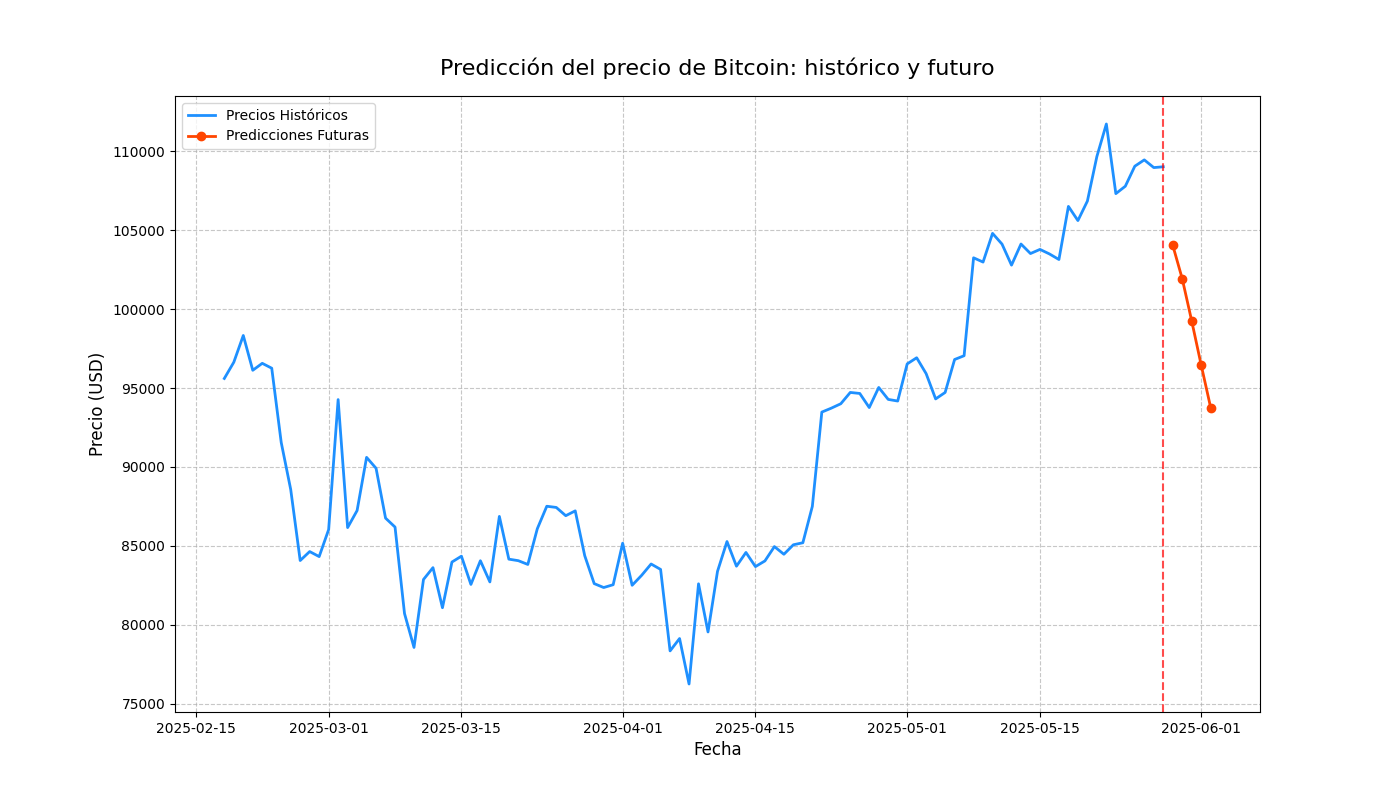
\includegraphics[width=0.85\textwidth]{../results/grafico_predicciones_futuras.png} % TODO: update
\caption{NHiTS - Predicción vs Real en los últimos 5 días}
\end{figure}

%%%%%%%%%%%%%%%%%%%%%%%%%%%%%%%%%%%%%%%%%%%%%%%%%%%%%%%%%%%%%%%%%%%%%%%%

\newpage
\section{Conclusiones}
\label{sec:conclusiones}

\subsection{Hallazgos Clave}

\begin{itemize}
\item El modelo ? superó al resto en todas las métricas evaluadas % TODO: update
\item Los modelos mostraron dificultades durante eventos de alta volatilidad
\item La arquitectura de atención demostró ser particularmente efectiva para capturar dependencias a largo plazo
\end{itemize}

\subsection{Limitaciones y Trabajo Futuro}

\begin{itemize}
\item \textbf{Limitaciones}:
\begin{itemize}
\item Sensibilidad a cambios bruscos de tendencia
\item Dependencia de hiperparámetros
\end{itemize}

\item \textbf{Mejoras propuestas}:
\begin{itemize}
\item Incorporar datos de redes sociales (sentiment analysis)
\item Ensamblar múltiples modelos
\end{itemize}
\end{itemize}

%%%%%%%%%%%%%%%%%%%%%%%%%%%%%%%%%%%%%%%%%%%%%%%%%%%%%%%%%%%%%%%%%%%%%%%%

\newpage
\section*{Anexo}
El código completo se encuentra disponible en: \\
\url{https://github.com/BenjaSar/AdST2}

\end{document}